\documentclass[tcn = 37075, sheet = false, abstract = false]{mcmthesis}
\problem{C}
\usepackage{palatino}
\usepackage{mwe}
\usepackage{slashbox}
\usepackage{algorithm2e}
\usepackage{mathrsfs}
\usepackage{xcolor}
\usepackage{graphicx}
\usepackage{caption}
\usepackage{float}
\usepackage{subcaption}
\usepackage{multirow}


\title{Understanding Employee Churn based on Information Accumulation and Bayesian Learning}
\author{}
\date{}
\begin{document}
\maketitle
\begin{abstract}
Network science is playing an increasingly powerful role in understanding human resource organizations, where various and complex network structures are rooted. Building up a network-based framework is always essential for further insightful analysis. Within such framework, specific models suiting corresponding needs can work wonder (yongci, gai).

In this paper, we construct an information network based on the organizational structure. Building on this network, we first model churn and the HR manager’s behaviors respectively. For the churn part, we derive a simple but effective model inspired by Bayesian learning. We capture staff members’ decision-making process through modeling information flow within network and learning mechanism after receiving information. For the HR manager part, we lay out five strategies he may use to fill the vacancies, with different strategies stressing on different rules of selection.

Next, we run various sets of simulations using our model. Through these simulations, we reproduce the current situations of ICM and the issues it is facing vividly, and meanwhile make plausible predictions of the effects of different changes (yuyan, songtui). For task 2, we first define a measure of productivity, then we detect how churn will affect it. Furthermore, we divide this effect into one part direct and the other indirect (be specific, yuchuan). We calculate the training cost and recruiting cost using the simulation results, solving task 3. Task 4 and task 5(songtui, be specific). 

To add richness to our model, we point out several practical extensions if given empirical data. Namely we can take into consideration the difference between information, the compatibility between staff members and positions, and the “celebrity” effect of the senior’s churn. We also illustrate how three crucial considerations, shared cognition, team training and stimulus of new staff member, from team science, can be incorporated. After that, we put out how other network layers can be considered together with information network, conceptually. At last, we test the sensitivity of an important parameter and analyze the strengths and weaknesses of our model.

%%%%%%
Network science is critical to 
Since the organization re

In this paper, we construct a Human Capital network according to the hierarchical organization structure of ICM and create a simple yet effective model to capture the dynamic processes, which includes organizational churn, promotion, and recruitment. For organizational churn, we propose and implement our probabilistic churn model based on Bayesian learning principles, which estimates and updates the likelihood of individual churn using the Beta-Bernoulli distribution. Then we develop three promotion measures based on the priorities of experience, dissatisfaction, and centrality. Furthermore, we propose several methods for the HR manager to control the recruitment rate.


In summary, our model is practical and reliable for the human capital dynamic processes in reality

\end{abstract}



\setcounter{tocdepth}{2}
\tableofcontents

\section{Introduction}

Network science has gained its popularity in management science. Modeling issues on human resource organization is, at root, modeling on its networks. In this problem, we need to consider a specific phenomena, churn, in  ICM company. To fulfill this, we decompose the problem into several steps:

\begin{itemize}
\item Build up a human capital network structure using information provided. Use it as framework for further analysis.
\item Design a model capturing the mechanism of churn effect and design reasonable reactions of the HR manager, thus making the dynamic process of staff members churn and HR reacts operate.
\item Set parameters to simulate the current situation of ICM company. Set up measures for company health and test effects of various changes. Point out heuristics for the HR manager accordingly.
\item Incorporate ideas from team science into the model and point out the possibilities of analyzing from multilayer view.
\item Implement sensitivity test and analyze model strengths and weaknesses.
\end{itemize}

\section{Fundamental Assumptions}

\begin{itemize}
\item No staff naturally retire or get fired. Each staff member makes a decision whether to leave. The decision is made through making a probabilistic inference.
\item Beyond the visible organizational structure, there exists an information network.
\item A staff member's monthly decision ("to leave" or "to stay") acts as a piece of information and flows through the information network.
\item Individuals digest received information through a learning process. This learning mechanism will affect their decisions by changing the probabilistic distribution.
\item The HR manager can affect the number of people in the positions via different combined uses of promotion and recruitment. A combined use of promotion and recruitment, in this paper, is called a "strategy".
\end{itemize}

\section{Preliminaries}

\subsection{Allocation of Levels of Positions}

The first task of constructing the organizing network of ICM requires assigning positions to offices in a plausible manner. We analyze the organization and obtained a plausible assignment, on which we will build our information network.

To explain the assumptions clearly, we first define terms "tree" and "tier". Tree is defined to be the whole picture of the organizational graph. Entries are defined to be in the same tier if they are on the same horizontal line in figure 1. Thus we can see that the tree stems from the higher tier of CEO to the lowest tier of branches. The assumptions are as follows:

\begin{itemize}
\item Every senior/junior manager should have a clerk in his/her office for administrative tasks.
\item The level of position of a staff tend to be higher when his office is closer to the CEO in the organizational graph.
\item The level of position of a staff tend to be higher when his office is the root of divisions of more people.
\item The level of position of a manager cannot be lower than someone whose office belongs to a lower tier.
\item Research tasks should be conducted by experienced employees.
\end{itemize}

Thus we can get the following allocation table for the 370 positions:
\begin{table}[htb!]
\centering
\begin{tabular}{l|l|lllllll|l}   \hline
\backslashbox{Tier}{}& \backslashbox{Position}{level}&1&2&3&4&5&6&7&Total\\ \hline
1                  & CEO              & 2              & 0              & 0                      & 0                        & 0                    & 0                      & 2                    & 4     \\\hline
\multirow{7}{2pt}{2} & Research           & 1              & 0              & 0                      & 0                        & 2                    & 0                      & 1                    & 4     \\
                   & CIO                & 1              & 2              & 0                      & 0                        & 8                    & 0                      & 3                    & 14    \\
                   & CFO                & 1              & 2              & 0                      & 0                        & 8                    & 0                      & 3                    & 14    \\
                   & HR                 & 0              & 1              & 0                      & 0                        & 2                    & 0                      & 1                    & 4     \\
                   & VP                 & 2              & 0              & 0                      & 0                        & 0                    & 0                      & 2                    & 4     \\
                   & Facilities         & 1              & 0              & 0                      & 0                        & 2                    & 0                      & 1                    & 4     \\
                   & Sales Marketing    & 1              & 0              & 0                      & 0                        & 2                    & 0                      & 1                    & 4     \\\hline
 \multirow{9}{2pt}{3} & Networks           & 0              & 1              & 1                      & 0                        & 11                   & 0                      & 1                    & 14    \\
                   & Information        & 0              & 1              & 1                      & 0                        & 11                   & 0                      & 1                    & 14    \\
                   & Program Manager    & 0              & 1              & 1                      & 0                        & 6                    & 5                      & 1                    & 14    \\
                   & Production Manager & 1              & 1              & 0                      & 0                        & 10                   & 0                      & 2                    & 14    \\
                   & Plant Blue         & 0              & 1              & 1                      & 0                        & 6                    & 5                      & 1                    & 14    \\
                   & Plant Green        & 0              & 1              & 1                      & 0                        & 6                    & 5                      & 1                    & 14    \\
                   & Regional           & 0              & 1              & 1                      & 0                        & 6                    & 5                      & 1                    & 14    \\
                   & World Wide         & 0              & 1              & 1                      & 0                        & 6                    & 5                      & 1                    & 14    \\
                   & Internet           & 0              & 1              & 1                      & 0                        & 6                    & 5                      & 1                    & 14    \\\hline
4                  & Director           & 0              & 6              & 6                      & 0                        & 6                    & 0                      & 6                    & 24    \\\hline
5                  & Branch             & 0              & 0              & 11                     & 25                       & 12                   & 120                    & 0                    & 168   \\ \hline

&Total              & 10             & 20             & 25                     & 25                       & 110                  & 150                    & 30                   & 370 \\  \hline
\end{tabular} 

*1:Senior Manager 2:Junior Manager 3:Experienced Supervisor 4:Inexperienced Supervisor 5:Experienced Employee 6:Inexperienced Employee 7:Administrative Clerk

\caption{The distribution of staff in different positions}
\end{table}

\subsection{Building up Information Network}

We set up to build the information network in this company. Define $V(G)=\{v_1,v_2,...v_{370}\}$ as the set of all positions. Each node denotes one position. Define $E(G)$ as the set of edges in the network. $(v_i,v_j)\in E(G)$ if at least one of the following holds:

\begin{itemize}
\item $i$ and $j$ are in the same office. Here one entry in figure 1 is considered as an office, whether it consists of two divisions of 14 staff members or only four staff members.
\item $i$ is the head of an office and $j$ is the head of the directly-related upper office or the opposite. Here the staff member in the highest level of position within an office is considered as the head of the office, such as the junior manager in Networks office and the experienced supervisor in Branch office.
\item $i$ and $j$ are both senior manager or junior manager.
\end{itemize}

$G=\{V(G),E(G)\}$ is the the graph of this network. We then visualize the network in the following picture (figure 1).

\begin{figure}[htb!]
\small
\centering
\includegraphics[width=14cm]{figure_2.png}
\caption{Information Network in ICM} \label{fig:Information Network in ICM}
\end{figure}

We calculate some properties of this network:

Then we turn to the main part of building up our model and using it for analysis. To deal with the complicated real problems, we first simplify them into two process. The first process is named as "output" and the second process is named "input". Like in the real world and in the problem, the "output" process refers to the situations where the staff leave his or her position. The "input" process, accordingly, refers to the combination of internal promotion and outsourcing recruitment. The formal models are presented in the next section. Based on this process division, we can easily see that the "input" process is where the Human Resource manager works his or her power to control and improve the company's current position.

\subsection{Terms and Notations}

In order to keep clear and consistent through the paper, we will settle down some fixed terms referring to some specific constituents. Besides, we will settle down some abbreviations for later use. The mathematical notation rules are also summed up in this section.

\paragraph{Terms and Abbreviations}
\begin{itemize}
\item Position: We use position to refer to all the nodes in the network.
\item Level of position: we use level of position to refer to the seven administrative levels (manager, supervisor or employee).
\item Abbreviations: we assign each level an abbreviation: SE-Senior Executive, JE -  Junior Executive, ES - Experienced Supervisor, IS - Inexperienced Supervisor, EE - Experienced Employee, IE - Inexperienced Employee, AC - Administrative Clerk
\end{itemize}

\paragraph{Mathematical Notation Rules}
\begin{itemize}
\item $t$: time is discrete and the minimum time interval is one month.
\item $\Omega^{(t)}$: the set of people who leave the company at the end of $t$. \item $\Theta^{(t)}$: the set of people who are recruited the company at the beginning of $t$. 
\item $\Gamma^{(t)}$: the set of people who work in the company at the beginning of $t$ after recruitment. It's obvious that the relation $\Gamma^{(t+1)}=\Gamma^{(t)}\bigcup \Theta ^{(t+1)} \backslash \Omega^{(t)}$ holds.
\item $f^{(t)}$: the mapping from $\Gamma^{(t)}$ to $V(G)$, which maps individual $i\in \Gamma^{(t)}$ to his position $f^{(t)}(i) \in V(G)$ at time $t$. $f^{(t)-1}$ is the inverse mapping.
\item $d(u,v)$: the distance between two nodes $u, v\in V(G)$, defined by the length of the shortest path connecting $u$ and $v$ in the graph.
\item $d_{ij}^{(t)}$: the distance between two individuals $i, j\in  \Gamma^{(t)}$ at $t$, defined by $d(f^{(t)}(i),f^{(t)}(j))$.
\end{itemize}


\section{Models}

(\textcolor{red}{need refinement}) We hold the intention to create a dynamic model which can be controlled by manipulating some of the parameters. Specially, we assume that the "output" process is largely determined by individual characteristics rather than company's policy. However, we also want to create a set of tools that human resource managers can use to deal with the possible staff problems. With these in mind, we design two models that capture the process of "output" with different emphasis and simulate three possible strategy for the human resource manager: purely recruiting, purely promoting and the "greedy" strategy. These models and simulations will help to solve the task 1-5 and even dig deeper insights about staff management. 

Before delving into the details of our models, we make some bold assumptions:
\begin{itemize}
\item We assume that all the data given in the first table in the problem, whether it is mean or average, has no uncertainty. That is the mean or median salary or recruiting cost is a certain number in our model.
\item We assume that the information will only transmit through the information web we have set up.
\end{itemize}

\subsection{Churn Model}

\subsubsection{Preliminaries}

In recent studies, Bayesian learning has been used to analyze information aggregation in social networks\cite{acemoglu2011bayesian}\cite{gale2003bayesian}, in which individuals modify their decision based on previous outcomes of other individuals in the network. 

For the sake of explaining our intuition, let us consider a simple Bayesian learning process. Suppose an random variable $u \in \{0, 1\}$ is drawn from a Bernoulli distribution, where the $p$ is unknown:
\begin{equation}
u \sim \mathrm{Bernoulli}(u; p) = p^u(1-p)^{1-u}
\end{equation}
Assume an observer wants to estimate the parameter $p$ by drawing multiple $u$s. The individual has a prior estimation $f(p)$ on $p$, which is described as a Beta distribution\footnote{The Beta distribution is chosen because it is the conjugate prior of the Bernoulli distribution. For more information on conjugate distributions, please refer to  \cite{bishop2006pattern}}
\begin{equation}
 f(p) = \mathrm{Beta}(p; \alpha, \beta) = \frac{p^{\alpha - 1}(1-p)^{\beta - 1}}{\mathrm{B}(\alpha, \beta)}
\end{equation}
where $\mathrm{B}(\alpha, \beta)$ is the normalization constant.
When seeing an outcome of $u = 1$, the observer updates his prior according to the Bayes' law\footnote{We ignore the normalization constants for simplicity.}: $f(p) \sim (p^{\alpha-1}(1-p)^{\beta-1}) \cdot p \sim p^{\alpha}(1-p)^{\beta-1}$, which can be viewed as increasing $\alpha$ by $1$. Similarly, the observer increases $\beta$ by $1$ if an outcome of $u = 0$ is seen. A simple analysis will show that if the number of observations reaches infinity, $\alpha / \beta \rightarrow p$, whereas the Beta distribution in this case reduces to a Dirac delta function $\delta(x - p)$, indicating that the observer's estimation converges to the correct $p$, regardless of the original prior.

\subsubsection{Modeling the Churn Rate}

In the light of this, we introduce a novel method to model the churn rate, which is conceptually similar to the above Bayesian learning process. Specifically, we view leaving the position as a decision making process: suppose an individual $i$ decides whether \textit{to leave} or \textit{to stay} in a particular month $t$ based on a random variable $u_{i,t} \in \{0, 1\}$, where $u_{i,t} = 0$ indicates \textit{to leave}, and $u_{i,t}=1$ indicates \textit{to stay}. 

$u_{i, m}$ is drawn as follows: First, we assume two hyperparameters $\alpha_{i, t}$ and $\beta_{i, t}$ for $i$, and draw $\displaystyle   p_{i, m} \sim \mathrm{Beta}(\alpha_{i, t}, \beta_{i, t})$; then we draw $\displaystyle u_{i, t} \sim \mathrm{Bernoulli}(p_{i, t})$; finally, we determine $i$ is \textit{to stay} if $u_{i,t}=1$; \textit{to leave} otherwise.

Integrating out the random variable $p_{i, m}$, we notice that the distribution of $u_{i, t}$ is a specification of the Beta-Binomial distribution with mean $\alpha / (\alpha + \beta)$ and variance $(\alpha\beta)/((\alpha+\beta)^2)$, which has some nice properties for modeling the churn process: on the one hand, we can easily estimate $i$'s probability \textit{to leave}, which is equal to $\beta_{i, t}/(\alpha_{i,t}+\beta_{i,t})$; on the other hand, an increase in $\alpha_i$ decreases $i$'s tendency \textit{to leave}, while an increase in $\beta_i$ increases the tendency \textit{to stay}. However, three problems remain: How to determine the prior $\alpha_i$ and $\beta_i$? How to update the hyperparameters? How to take the network structure into account?

\paragraph{Determining the Prior} Given a churn rate $p$, we can easily model the effect of a churn rate of $p$ per year by setting $\beta / (\alpha + \beta) = p / 12$. We further observe that the variance of the Beta distribution is $\displaystyle \frac{\alpha\beta}{(\alpha+\beta)^2(\alpha+\beta+1)}$, so that larger $(\alpha + \beta)$ leads to smaller variance, indicating better estimation of $p$, and more knowledge to the company status. Thus, it is safe to assume that people on high level positions have a larger $(\alpha+\beta)$ compared to others, and their decisions are less volatile.

\paragraph{Updating $\alpha_i$ and $\beta_i$} We notice that in ICM, an individual is more likely to churn if he/she is connected to other individuals who have churned. This can be described as a learning process for the individual: each month, he/she observes the decision made by other individuals in last month. For every observation of "to stay", the individual increases his/her $\alpha$; for every observation of "to leave", the individual increases his/her $\beta$. We normalize the update values, so that every month, an individual's $(\alpha+\beta)$ increases by 1.

\paragraph{Information Reduction} The impact of churn information vary upon the distances between the source and destination. From an individual's perspective, the resignation of someone in the same department should have a greater impact than that of someone from another department. We take this into account by reducing the update value of the hyperparameters. Empirically, we reduce the update by $d^2$ if the information takes at least $d$ steps to transmit. 

\subsubsection{An Algorithm for the Churn Model}
To summarize, we introduce an algorithm for this process for every individual $i$:
\begin{itemize}
\item Sample the churn result for month $t$ using hyperparameters $\alpha_{i,t}$ and $\beta_{i,t}$, and determine whether to stay or to leave;
\item If $i$ decides to stay, initialize two variables $\hat{\alpha}$ and $\hat{\beta}$ for update;
\item For every individual $j$ in $\Gamma^{(t)} \backslash \Theta^{(t)}$(individuals who stays), update $\displaystyle \hat{\alpha} = \hat{\alpha} + \frac{1}{d_{ij}^{(t)}}$;
\item For every individual $j$ in $\Omega^{(t)}$, update $\displaystyle \hat{\beta} = \hat{\beta} + \frac{1}{d_{ij}^{(t)}}$;
\item Update $\displaystyle \alpha_{i,t+1}=\alpha_{i,t}+\frac{\hat{\alpha}}{\hat{\alpha}+\hat{\beta}}$, and $\displaystyle \beta_{i,t+1}=\beta_{i,t}+\frac{\hat{\beta}}{\hat{\alpha}+\hat{\beta}}$
\end{itemize}


\subsection{Vacancy Filling Models}

After modeling the churn process, we need to consider the strategic process of filling the vacancy from the perspective of the HR manager, which combines promotion strategies and recruitment strategies. Since recruitment a higher level position usually requires more time and money compared to promoting a low-level employee and then recruit for that vacancy, a rational HR would always prefer promoting to recruiting whenever possible. This allows us to consider these two aspects separately.

\begin{itemize}
\item He has a maximum possible effort to recruit. He cannot post more recruitment than this maximum because of his ability and resource limit. The maximum effort is not affected when there vacancy in HR office. 
\item When the number of vacant positions is higher than his maximum, he ranks the vacant positions from higher level to lower level. That is to say, he will first consider recruiting a manager rather than an employee when they are all vacant. The motivation behind this lies in that the time needed for recruiting a manager is much longer.
\item He can only renew his recruitment post over a length of period, e.g. quarterly or semi-annually.
\end{itemize}

\subsubsection{Promotion Models}
We summarize some basic rules for promotion:
\begin{itemize}
\item The HR manager does not read the annual evaluation report, thus does not know anything about the matching between staff and positions. In this way, he/she will not consider changing staff within one level.
\item His/Her first choice is to promote someone that has reached the experience requirement to fill the vacancy. If no person is qualified and recruiting resources are permitted, he/she will then post recruitment need for this position on the next.
\item If during the time the recruitment need is posted, he finds that there is one person's experience has reached the requirement. He will directly promote and cancel the recruitment post.
\item He will not promote a clerk because recruiting an inexperienced employee is cheaper and less time-consuming than recruiting a clerk. In other words, a "naive" manager never promotes a clerk.
\end{itemize}

Under current situations, the HR has no knowledge about the capabilities of an employee, nor their probability to leave. Therefore, to make the promotion process \textit{fair}, the HR should choose the employee on the lower level with the longest working experiences. Hence, we have the following strategy:
\paragraph{Experience Oriented} For a vacancy on level $l ~~ (l < 6)$, select the employee on level $l+1$ with longest working experiences; the employee should also satisfy the promotion requirements. If nobody is available, start recruiting this position.

If the HR happens to learn the churn model previously mentioned, he can make inference on the probability of churn of a individual, thus introducing a slight improvement over the experience oriented model:
\paragraph{Dissatisfaction Oriented} For a vacancy on level $l ~~ (l < 6)$, select the employee with the largest $\beta / \alpha$(or the highest churn probability) among all the employees on level $l+1$ who satisfy the promotion requirements. If nobody is available, start recruiting this position.

The HR can also consider the network structure by promoting the employee with the largest centrality:

\paragraph{Centrality Oriented} For a vacancy on level $l$, select the employee with the largest closeness centrality(tends to be greater when the employee is in the middle of the network) from the qualified employees on level $l+1$. If nobody is available, start recruiting this position.


\subsubsection{Recruitment Models}
We make the following assumptions on the recruiting strategies:
\begin{itemize}
\item The HR has a maximum possible effort to recruit. He cannot post more recruitment than this maximum because of his ability and resource limits. The maximum effort is not affected when there is vacancy in HR office. 
\item When the number of vacant positions is higher than the maximum effort, he ranks the vacant positions from higher level to lower level, and only try to recruit the positions with the highest levels. In other words, he will prioritize recruiting a manager over recruiting an employee. 
\item He can only renew his recruitment post over a length of period, e.g. quarterly or semi-annually.
\end{itemize}

Thus, the HR manager has two direct means to increase the recruitment rate: he can either increase the resource limits, so that more people will be recruited in a fixed time period, or simply increase the frequency of the renewal of his recruit post. Also, the HR can control the promotion rate by setting different thresholds for promotion, which is also an indirect method of controlling recruitment. 



\subsection{Model Functions and Modifications}

Till now, our models have already encompassed a large variety of mentioned features in ICM company, including:

\begin{itemize}
\item The information web captures how "churn" diffuses among staff members.
\item The risk of churn can be identified in early stage by observing each staff member's $\beta/\alpha$. The higher $\beta/\alpha$, the more likely the staff member chooses to leave.
\item The resignation of one employee will increase the $\beta$ parameter of other employees, thus increasing their chance of resigning.
\item We treat the fact that churn rates for middle managers are higher than other levels of positions by allowing different priors $\alpha$ and $\beta$ for different levels.
\item HR can use the resource limits, recruitment time period, and promotion threshold to control the recruitment flow.
\end{itemize}

However, the models can be extended to reflect more subtle aspects about the company. Simulations for these might not be meaning for the lack of real data. We present the ways that it can be enriched and once we have real data, they can be realized.


\paragraph{Matching and Frictions} 

Our models can reflect the issues related to the compatibility between staff and positions by introducing new assumptions into it. To get insight  about how this works, we can see the following toy model. 

We can assume there are positions needing two types of skills, represented by {0, 1}. There are also two kinds of people, the person having {0, 1} skills. If the person is matched with the position, he will have higher productivity. If the HR manager has no information about what kind of skill each staff member has, the distribution of people on positions will be random and half of the people match with their positions and half not. By reading annual report, HR can know about what kind of skill a staff member has. In other words, the HR manager can distinguish a staff member's skill after he has been in the company after 12 months. Then when considering his strategy, the HR manager can take the compatibility between people and positions into consideration.

This is matching can come into our models. The more detailed classification on the people and skills, the more subtle aspects of matching we can reflect. The way we reflect them is simply by changing the strategy for the HR manager accordingly. Again due to lack of more information, we don't want to go into details in this part. But if given more information about the real company and more time we can enrich our model and ch our models and simulate the matching effect.

\paragraph{Information Intensity} 

People in different levels of positions have different impacts on other staff members. In most cases, we cannot expect the resign of the leader of your office and the leave of an office mate having the same impact on you. The higher the level people are in, the more "powerful" his choice is likely to be. We can take this into consideration using our model by introducing a set of parameters: information intensity. Suppose each level of position has a certain "information intensity". If, suppose the information intensity for a clerk is 1, the information intensity for a senior manager might be number like 20. In generalization, we can assume the information intensities are $II_i, i=1, 2, ..., 7$ and normalize it to $II_7 = 1$. 

Empirically, we can estimate the parameters depicting information intensities reasonably. Based on our model, given all past information before $\tau$ within the company, we can calculate the probability that each individual
will resign at $\tau$. If we incorporating information intensities, thees probabilities will be a function of $II_i, i=1, 2, ..., 7$. Then we will solve the following maximum likelihood estimation (MLE) problem:

$$\max\limits_{\{II_i\}_{i=1}^7} \prod\limits_{\tau=t-N}^{t-1}\{\prod\limits_{i \in \Omega^{(\tau)}} p_i^{(\tau)} \prod_{i\in \Gamma^{(\tau)}\backslash \Omega^{(\tau)}}(1-p_i^{(\tau)}) \}$$

We can take natural log logarithm of the equation and then adopt Gradient Descent algorithm to find the optimal solution. 

%Both in reality and in the context of this problem, a certain amount of experience is required for getting promotion. Usually, the higher tier to be promoted into, the longer the experience is needed. In the model, we assume that the required experience for promotion only takes into account the time length of being in the former level. E.g. only the time length of being in the level of junior manager set to be requirement for consideration of promoting senior manager. Suppose the experience requirement for each level of position is represented by $R_i, i = 1, 2...,7$. This can be a rich set of tools that the HR manager can use to control the organizational structure and even churn rate.


\section{Simulations}

\textbf{Added Assumptions for Simulations}

In order to get reasonable simulation results, we settle some parameters. This, on the one hand offers ease for simulation, while on the other land, does not lose its closeness to reality. Our added assumptions for parameters:
\begin{itemize}
\item The required experience for the seven levels of positions are 48 months, 48 months, 24 months, 24 months, 12 months, 0 month respectively (from higher position to lower position).
\item The time period for updating the recruitment post is 6 months.
\item The $\alpha$ and $\beta$ for different levels of positions are(levels in decreasing order)144, 120, 64, 48, 32, 24, 24.
\item The maximum recruiting effort for the HR manager is 9\% of 370 (average of 8\%-10\%) for most cases. Any change in this parameter will be mentioned.
\end{itemize}

\subsection{Task 1: Simulations with Current Situation}

In this section, we first present our basic simulation results of current situation. The boxplot below shows the churn rate in different level of positions in 50 simulations. The churn rate of middle-manager (JE, ES and IS) is roughly 30\% and the churn rate for other positions (SE, EE, IE and AC) is around 15\%. The overall churn rate of the company is relatively stable at 18\%, which can accurately depict the current situation of ICM.

\begin{figure}[htb!]
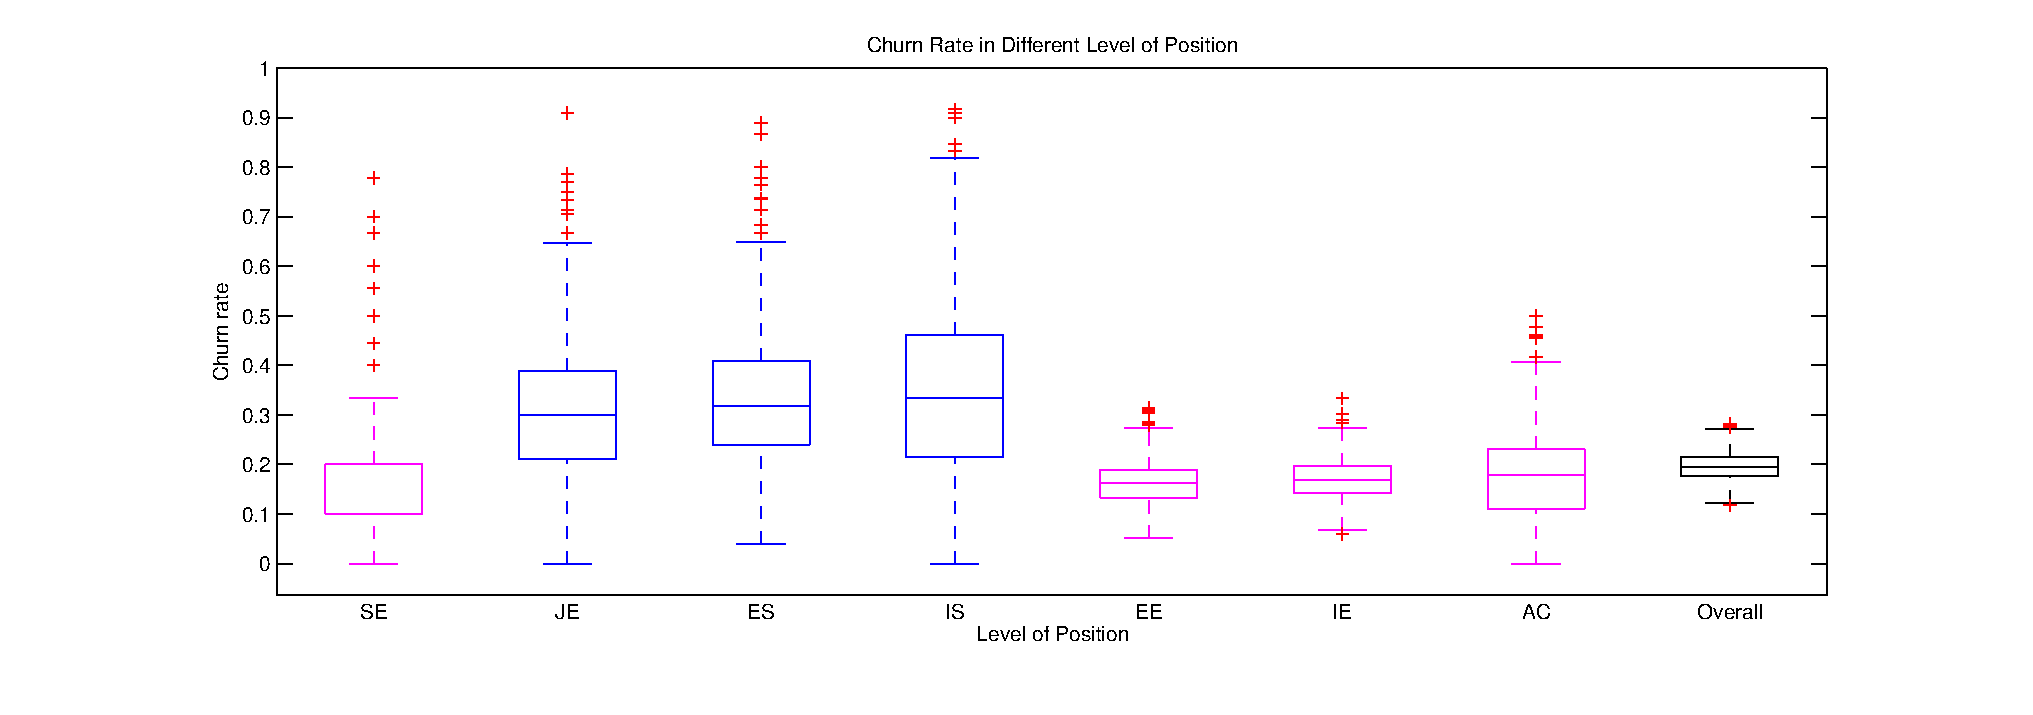
\includegraphics[width=16cm]{task1_2.eps}
\caption{Churn Rates of Different Level of Position} 
\label{fig:2}
\end{figure}

Another feature of ICM is churn rate is steadily increasing. The simulation result does exhibit similar trend. We show the overall churn rate in next five years below.

\begin{figure}[htb!]
\centering
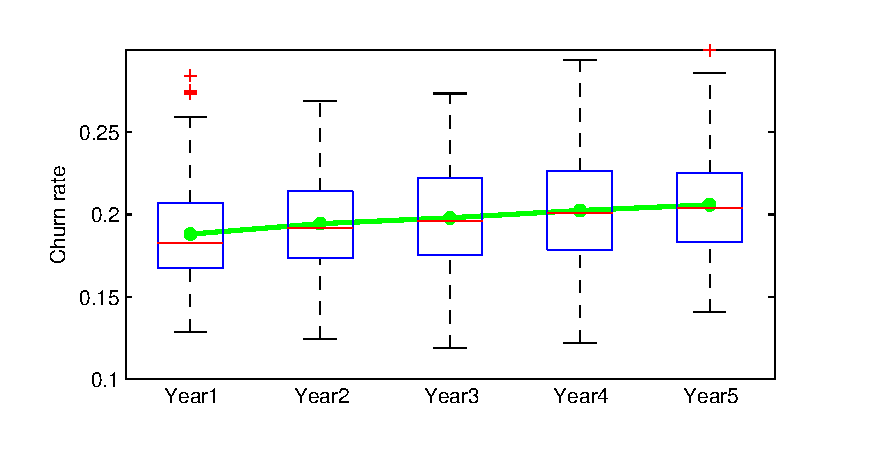
\includegraphics[width=9cm]{task1.eps}
\caption{Overall Churn Rates in Next Five Years} 
\label{fig:2}
\end{figure}

In spite of a couple of outliers, the major trend can be easily seen in the boxplot. The median value of churn rate has shown a slow but steady increase, from 18\% in the first year to 20\% in the fifth year.

\subsection{Task 2: Defining Productivity and Testing Churn Influences}

To define a metric to measure this company's organizational productivity, we start from the individual level. This metric should incorporate the following three aspects:

\paragraph{Position Level}
Different levels of position surely make different contribution to the overall performance of a company. We reasonably assume the relative average annual salary of $i$'s position level, $S_i^{(t)}$ can properly reflect his actual level contribution.

\paragraph{Training experience}
Experience in his current position definitely contribute to one's productivity. We use the training cost the company spent on the individual since he began working in the current position as a proxy of his experience, denoted by $T_i^{(t)}*t_i^{(t)}$.

\paragraph{Dissatisfaction}
An individual more unsatisfied with current situation tends to work less inefficiently, leading to lower productivity. We calculate $i$'s dissatisfaction $\sigma_i^{(t)}$ as:

$$\displaystyle \sigma_i^{(t)}=\sum_{\tau=t-t_i^{(t)}+1}^{t-1}e^{-(\tau-(t-1))}\sum_{j\in \Omega^{(\tau)}}\frac{1}{d_{ij}^{(\tau)2}}$$

We normalize $\sigma_i^{(t)}$ to the form of $\frac{1}{1+\alpha\ln{(1+\sigma_i^{(t)})}}$. $\alpha$ is a parameter reflecting the influence of dissatisfaction. We set $\displaystyle \alpha = 0.1$ in the following calculation in this part. We will carry on sensitivity analysis regarding to this parameter in later section.\\

Incorporating the three components, the productivity of an individual $i$ at time $t$ is:
$$ p_i^{(t)}=\frac{1}{1+\alpha\ln{(1+\sigma_i^{(t)})}}(S_i^{(t)}+T_i^{(t)}*t_i^{(t)})$$

To calculate organizational productivity, we use weighted sum of individual's productivity. The weight $w_i^{(t)}$ is determined by information network structure. An individual in an important position weighs more. Here we use \textit{closeness centrality} to reflect this importance. So organizational productivity is defined by:

$$\displaystyle P^{(t)}=\sum\limits_{i\in\Gamma^{(t)}} w_i^{(t)}*p_i^{(t)}=\sum\limits_{i\in\Gamma^{(t)}}p_i^{(t)}\sum\limits_{v\in V(G)\backslash f^{(t)-1}(i)}\frac{d(v,f^{(t)-1}(i))}{370-1}$$

Using this measure, we can track the dynamic change of organizational productivity. We can distinguish two kinds of effect associated with an individual's resign:

\paragraph{Direct Effect} The productivity of resigned individuals.
\paragraph{Indirect Effect}
The loss of productivity caused by the increase of dissatisfaction of the remaining staff in this company after the resign.

$$DE^{(t)}=\sum\limits_{i\in\Omega^{(t)}}w_i^{(t)}*p_i^{(t)}$$ $$IE^{(t)}=\sum\limits_{i\in\Gamma^{(t)}\backslash\Omega^{(t)}} w_i^{(t)}*(\frac{1}{1+\alpha\ln{(1+e^{-1}\sigma_i^{(t)})}}-\frac{1}{1+\alpha\ln{(1+\sigma_i^{(t+1)})}})(S_i^{(t)}+T_i^{(t)}*t_i^{(t)})$$

We now calculate the loss of organizational productivity associated with a person's resign and decompose it into direct and indirect effect. We run our simulation over next five years for 50 times and average the results for presentation.

\begin{figure}[htb!]
\centering
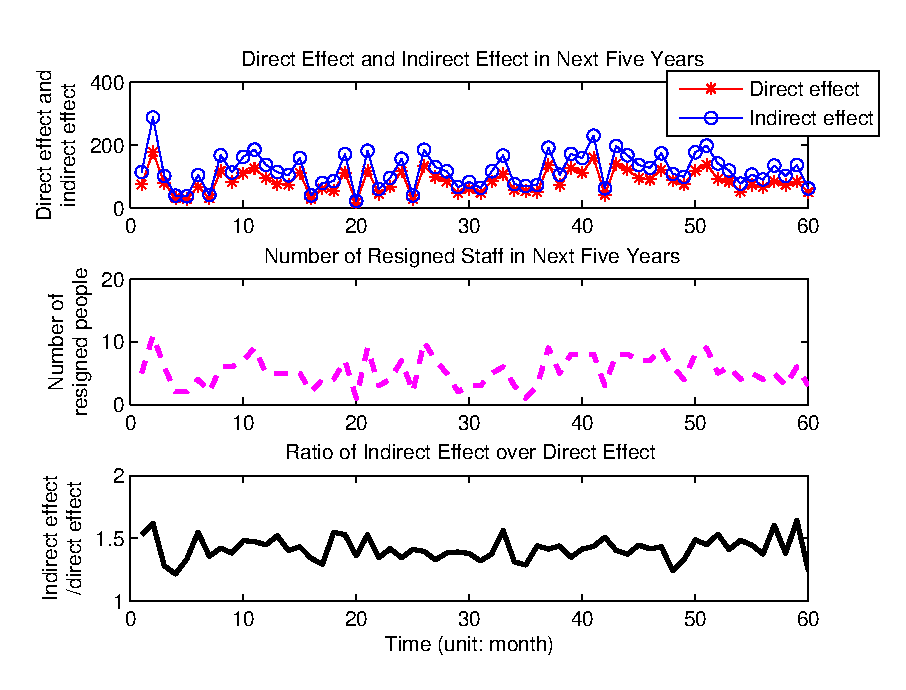
\includegraphics[width=14cm]{Productivity_figure.eps}
\caption{Effect on Organizational Productivity} 
\label{fig:3}
\end{figure}

It's obvious direct and indirect effect on organizational productivity closely follow the number of resigned staff. An individual's resign will cause about 20 units of direct effect and 25 units of indirect effect. Total organizational productivity is 2000-2500 units monthly, so a person's resign costs 2\% of total organizational productivity.

Another observation is the ratio between indirect and direct effect. In the simulation, the former is larger than the later with a stable ratio. The parameter $\alpha$ can reflect how a person view the resign of another individual and we will return to it later.

\subsection{Task 3: Budget Calculation}

We now consider the budget of the company related to human capital. The budget consists of three components: staff salaries, recruitment cost and training cost. To make calculation easier, as we assumed before, all individuals in the same position level have the same salary and training cost, and recruitment cost is uniform in each position level. All costs are incurred uniformly distributed across the corresponding time span.

We run simulation of the company and show the calculated cost below:

\begin{figure}[htbp]
\begin{minipage}[t]{0.5\linewidth}
\centering
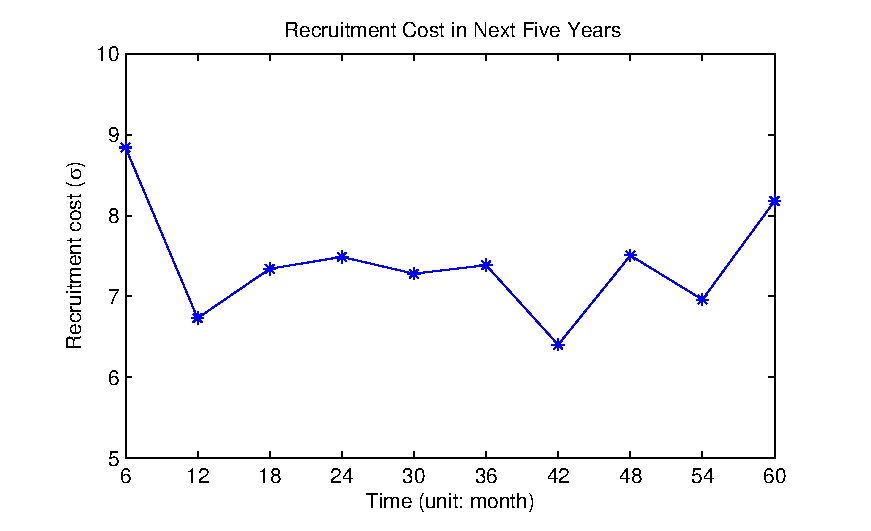
\includegraphics[width=1.0\textwidth]{Recruitment_Cost.eps}
\end{minipage}%
\begin{minipage}[t]{0.5\linewidth}
\centering
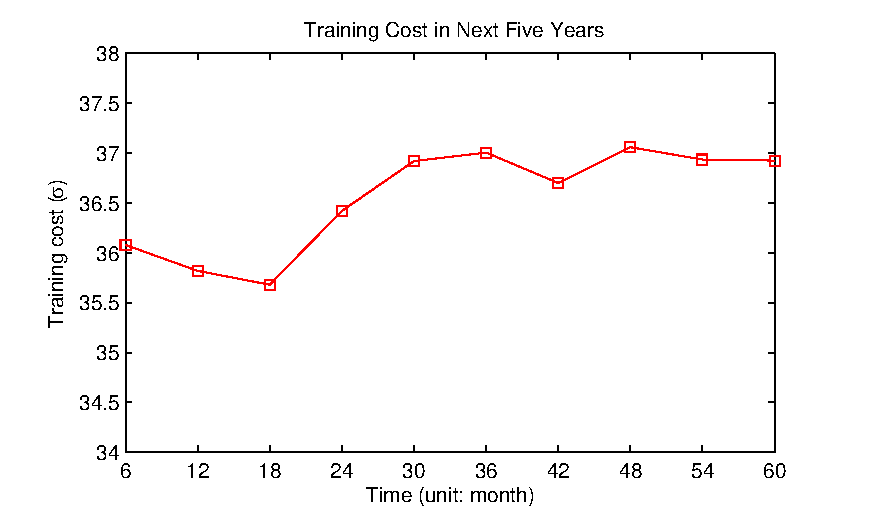
\includegraphics[width=1.0\textwidth]{Training_Cost.eps}
\end{minipage}%
\caption{Budget Calculation for Next Five Years}
\end{figure}

The cost presented is calculated every six months. On average, the recruitment cost and training cost is approximately $7\sigma$ and $37\sigma$ every six months respectively. However, they are only a small fraction of total cost, as we have not reported salary cost here, which accounts for the largest part.

\subsection{Task 4: Changing Churn Rate}

In this part, we simulate the company under different churn rates. We assume an increase in average churn rate from current 18\% to 25\% and 35\%. To achieve this goal, we can simply adjust the $\beta$-to-$\alpha$ ratio: for a churn rate of 25\% per year, we let $\beta/\alpha = 0.25/12 = 0.02083$; for 35\% per year, we let $\beta/\alpha = 0.35/12 = 0.02916$.

We simulate fifty times for each churn rate. The following graph shows our results.\footnote{Due to limited space, we cannot provide full statistical results to prove that the churn rates of our simulation is indeed 25\% and 35\%; however, we can estimate that is the case using the following method: We observe that the recruitment rate is stable for different churn rates, thus the stable percent of employees with a 35\% churn rate should be around $80 \times 18 / 35 \sim 42$ percent. This is apparent in the top graph in Figure \ref{fig:2}.}
The three line charts reflect the evolution of staff number, monthly organizational productivity and monthly cost over next 20 years respectively under different churn rates. We take the average of ten simulations. The trend of these company characteristics is quite clear. The company is running on 80\% full status of positions, namely around 300, under 18\% churn rate over a long time span. However, its staff number declines dramatically during the first six years if churn rate increases to 25\% or 35\%. Then it gradually becomes stable and settles down at approximately 60\% and 40\% full status of positions when churn rate is 25\% and 35\% respectively.


\begin{figure}[htb!]
\centering
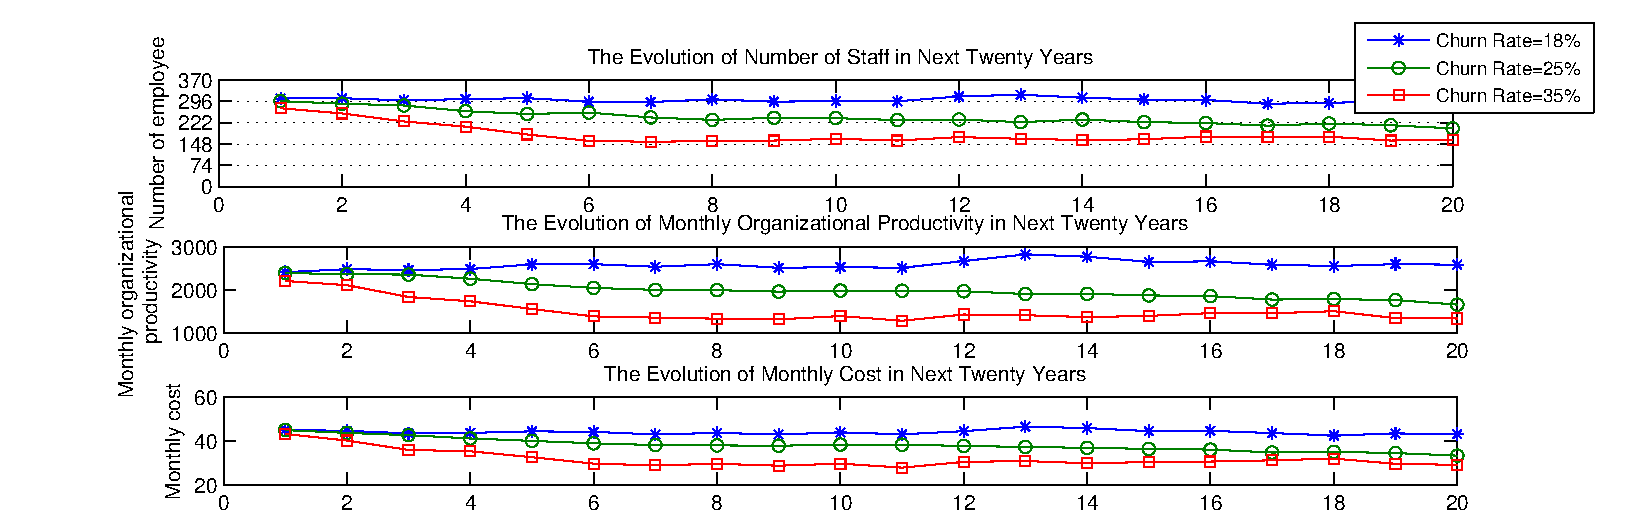
\includegraphics[width=16cm]{Task4_1.eps}
\caption{Evolution of the Company in Next Twenty Years Under Different Churn Rates} 
\label{fig:2}
\end{figure}

The trend also applies to organizational productivity and cost. Under high churn rate, more people are leaving the company, leading to  both higher direct and indirect effect. So organizational productivity decreased by around 30\% and 50\%. Salary accounts for the largest part of cost and training comes second. Although a high churn rate will incur higher recruitment cost, it is minor compared with the large decline on salary and training cost resulted directly from fewer staff. Cost decreases by nearly 20\% and 40\%.

To sustain in current percentage of status, HR manager should change the recruitment strategy. In our baseline simulation and all simulations followed, we assume the time period for updating the recruitment post is 6 months and the recruitment effort is 9\%. Now we need to change these two parameters to fill in the gap quickly. We change updating interval to 4 months and recruitment effort to 8.3\% under 25\% churn rate and 3 months and 9\% under 35\% churn rate to sustain 80\% full status for position. The boxplot below shows the distribution of the results from ten simulations:

\begin{figure}[htb!]
\centering
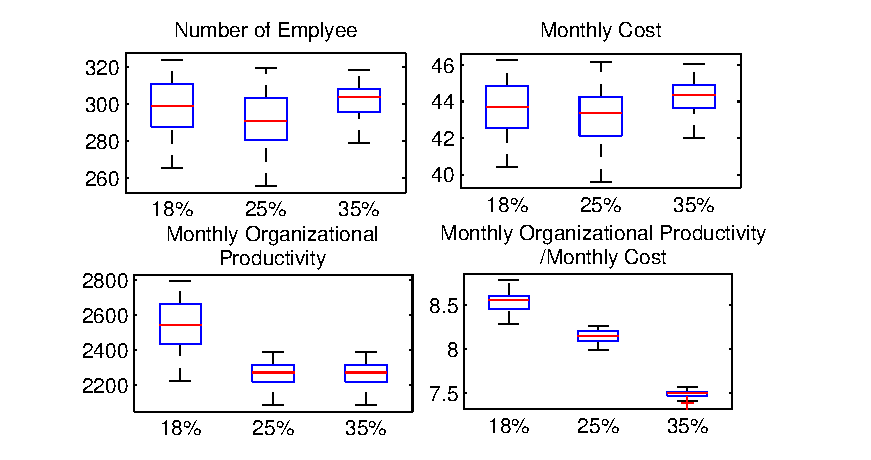
\includegraphics[width=15cm]{Task4_2.eps}
\caption{Comparison of Different Churn Rate under New Promotion Strategy} 
\label{fig:2}
\end{figure}

Under these new promotion strategies, the company can roughly sustain 80\% capacity. Its monthly cost presents no significant difference. However, organizational productivity vary a lot. It decreases by more than 10\% under high churn rate, even if the staff number remains the same. If we use organizational productivity per unit cost as an indicator of the company's efficiency on using money, we can see from the last boxplot that the company is running more efficiently under relatively low churn rate.

\subsection{Task 5: Pure Promotion and HR Health}
Having set up several scenarios to evaluate the impact of different churn rates, we now apply our methodology to help us identity the impact on human resource health with no external recruiting. Apparently, with a alarming churn rate, recruiting nobody will definitely result in a decrease in the number of employees, cost, and productivity, so our emphasis will be on the number of employees in different offices. We modify our model to eliminate external recruitment(thus allowing only churn and promotion), and estimate the percentage of the employees in the offices. For better estimation, we assume a uniformly random distribution on the years of experience for the employees, so that one-fourth of the employees in each level are qualified to promote.

We visualize our results in Figure \ref{fig:hr-health}. We found that the offices in tiers 1 and 2 sustains good health, whereas offices in lower tiers suffer significant reduction in HR health. This conclusion is rather counter-intuitive at first sight, since middle managers tend to have a higher churn rate, but quite plausible given that low-level positions are not supplied by recruitment, whereas high-level positions can be sustained by promotion.
We report that the number of remaining employees after 2 years is around 204 people, which is close to the theoretical value\footnote{The theoretical value is $370 \times 0.85 \times (1 - (325 \times 0.18 + 45 \times 0.30) / 370 )^2 = 204.01$}.

\begin{figure}[t!]
        \centering
        \begin{subfigure}[h]{0.45\textwidth}
                \includegraphics[width=\textwidth]{figures/0.pdf}
                \caption{Initially}
        \end{subfigure}%
        \begin{subfigure}[h]{0.45\textwidth}
                \includegraphics[width=\textwidth]{figures/12.pdf}
                \caption{After 12 months}
        \end{subfigure}
        \begin{subfigure}[h]{0.45\textwidth}
                \includegraphics[width=\textwidth]{figures/18.pdf}
                \caption{After 18 months}
        \end{subfigure}%
        \begin{subfigure}[h]{0.45\textwidth}
                \includegraphics[width=\textwidth]{figures/24.pdf}
                \caption{After 24 months}
        \end{subfigure}
        \caption{HR health in different periods. Darker colors indicate a office with higher percentage of employees. White indicates an 50 percentage.}
        \label{fig:hr-health}
\end{figure}


\subsection{Comparing among Strategies}

Now we aim to improve the current situation by adopting some alternative strategies. Currently, when deciding which one to promote among all qualified candidates, HR manager will choose the one with the longest working time (\textit{Experience}). We consider two other ways discussed before: selection by centrality within the information network (\textit{Centrality}) and selection by likelihood to leave (\textit{Likelihood}). We still use closeness centrality defined in previous sections.

\begin{table}[h]
\centering
\begin{tabular}{lllllll}
\hline
\multicolumn{2}{c}{Different Strategies}     & Year2   & Year4   & Year6   & Year8   & Year10  \\ \hline
Experience                  & Staff Number & 313.0   & 310.7   & 304.9   & 298.8   & 292.9   \\
\multirow{2}{*}{Centrality} & Staff Number & 311.1   & 307.5   & 302.0   & 295.7   & 290.0   \\
                            & Increase(\%) & -0.60\% & -1.04\% & -0.94\% & -1.01\% & -0.99\% \\
\multirow{2}{*}{Likelihood} & Staff Number & 311.1   & 309.1   & 308.4   & 303.7   & 300.6   \\
                            & Increase(\%) & -0.62\% & -0.52\% & \textbf{1.16}\%  &\textbf{1.64}\%  & \textbf{2.61}\%  \\ \hline
Experience                  & Productivity & 2574.9  & 2706.2  & 2698.5  & 2651.7  & 2612.8  \\
\multirow{2}{*}{Centrality} & Productivity & 2589.3  & 2789.0  & 2878.6  & 2897.0  & 2916.8  \\
                            & Increase(\%) & 0.56\%  & 3.06\%  & \textbf{6.67}\%  & \textbf{9.25}\%  & \textbf{11.63\%} \\
\multirow{2}{*}{Likelihood} & Productivity & 2577.8  & 2759.3  & 2872.8  & 2886.0  & 2904.0  \\
                            & Increase(\%) & 0.11\%  & 1.96\%  & \textbf{6.46}\%  & \textbf{8.84}\%  & \textbf{11.14}\% \\ \hline
\end{tabular}
\caption{Comparison among Different Strategies}
\end{table}

\section{Task 6: Extension - Team Science and Multilayers}
There are several possible extensions to the models we have described before. These extensions are used to modify some of the bold but kind of restrictive assumptions made before and help to come closer to reality. Note that some of these new extensions need information about the real data of the company. Besides, being more precise means in the other direction that the extended models will not be as powerful and encompassing as the baseline models. Though the insights they are shedding lights on are basically the same.

\subsection{Incorporating Team Science}

Recent studies on team performance have point out many possibilities to rigorously model teamwork.\cite{salas2008teams} There are many established findings from team science that can be merged into our models. The three most prospective ones are related to "shared cognition", "new-staff stimulus" and "team training". Here we point out the possibilities and define some of them informally. Incorporating them rigorously needs more modifications.

\subsubsection{Shared Cognition}

Shared cognition has been stressed by many researchers to be one of the crucial factors that shape the team performance \cite{cannon2001reflections}. One of the famous model is the Shared Mental Model (SMM) defined as a mental representation of knowledge regarding key components of a team's environment that is shared among team members\cite{nandkeolyar2008teams}. In order to work more efficiently, team members must predict what other teammates are going to do and what they need to do so, so that they can select actions that are consistent and coordinated with those of their teammates. \cite{mathieu2000influence}

Team cognition can form within different kinds of teams. In our context, a reasonable choice is an office. Staff working within an office share the same goal and shared cognition can positively contribute to its performance. Different measures have been developed to scientifically measure shared cognition\cite{cannon2001reflections}. We can take advantage of these measures to design an extension of our models. Especially when given empirical data (the time and numerical shared cognition), we can estimate the shared cognition growth model parameters using established models(\textcolor{red}{need citation}). We won't go into details on these measures or empirical methods. Instead, we put forward one measure within our context.

Consider an office $O$ with several individuals. . Define $t(i,j)$ as the length $i$ and $j$ has been working together. We can then use $\sum\limits_{i\in O}w_i\sum\limits_{j\in O\backslash \{i\}}t^2(i,j)$ as a measure of team cognition. The squared term can reflect the increasing speed of forming cognition and the weight reflect the relative importance.  Team cognition can be developed between two or three individuals.(\textcolor{red}{need citation}). So we assume team cognition is separable and additive and focus on interpersonal relation in pairs.

Another possibility is to use network and related concepts. We can define two individuals are connected if their co-working time is larger than a certain threshold. Then we can calculate measures such as the average degree in this network. Similarly, we can attach a weight to each edge according to how long they have been working together and build a weighted graph. We can use methods developed to study this teamwork network. We can also use the concept multilayer to combine this network with other kinds of network. We will return to multilayer network in next subsection.

%\subsubsection{Stimulus of New Staff Members}

%The second factor from team science that we can make use of is the stimulus of new team members. As illustrated in existing literature\cite{salas2008teams}, 

%This can be modeled by exerting a turbulence on the office performance when there is a new member coming into the office. 

\subsubsection{Team Training}

Another concept that we can potentially utilize in our models is team training. Currently, HR manager does not offer any training to the "team" or "office" as a whole. Like offering individual's training, we can take into account the team training. Being trained as a team can improve team members' understanding of each other's roles, promote teamwork and enhance team performance\cite{cooke2004advances}. We can view team training as an accelerator of team cognition development. So we can multiply the team cognition measure we developed before by a function of team training to reflect this effect. 

Adding this process will not directly affect the dynamic process of staff's leaving and HR manager's filling vacancy. However, it will affect the productivity of the company by promoting the efficiency of teamwork. This effect may change the decision making of HR manager with the aim to maximize organizational productivity per unit of cost. 

\subsection{Incorporating Multilayer Networks}

In this section, we will explore the progress made by recent studies about multilayer networks and apply this concept to our company context to help HR achieve better human resource management.

In previous sections, we have formulated a model based on the office organizing structure. This network describes how the churn information flows among all individuals. However,  interpersonal relationship is much more complicated. On the one hand, people are consistently entering and leaving the company, causing a change of structure in the network. On the other hand, people have different types of interaction, such as:
\begin{itemize}
\item People in the same office work as a team and usually cooperate with each other more frequently. 
\item People in the organizing structure have a administrative relation, which means an individual is directly supervised by the other.
\item People can be close friends with each other regardless of their positions.
\item People can have trust in his/her supervisors, and vice versa.
\end{itemize}

These interaction networks can provide us with more information, while shedding some light on more complex problems and enabling better solutions to problems that we are currently dealing with. Since we lack data on other layers of networks, it is impossible to implement a simulation. Hence, we provide some rules for connecting the information with other layers, as well as some solutions for better churn rate analysis.

\paragraph{Network based on position} Since the information network is already based on position, such networks can be easily connected by introducing coupling edges. A simple example is the supervision networks, which is a tree structure among different positions. Since supervision in office is a strong relationship, information transmitted through supervision is stronger than the average information network. Another example is the teammate relationship, where information is transmitted more frequently.

\paragraph{Network based on people} Some relationships - such as friendship and trust - depend on people. Friendship allows for the transmission of more personal information, and trust enables directed transmission of information. Both increases the transmission intensity of the information flow, for one tends to accept advice from friends and mentors more often. However, people can switch positions(or even leave) in the company, so maintaining a static network is unfeasible. One approach, however, is to introduce direct cross-layer links with length zero from a person node to a position node. A qualified HR should always track the person-position relationship and modify the structure of the network when necessary.

Now let us assume that we have incorporated teammate, friendship and trust relationship layers to our information network. We provide some improvements over our previous solution to churn rate analysis and productivity estimation.
\begin{itemize}
\item Apart from information flow, churn information can also transmit along other layers of networks;
\item We reduce our time slice from one month to a week, which allows more frequent information transmission between friends and teammates;
\item We increase the impact of turnover decisions made by trusted individuals;
\item We take friendship into account when calculating shared cognition, where friends in the same office tend to have increased shared cognition, and hence productivity.

\end{itemize}
\section{Sensitivity Analysis}

In this section, we implement sensitivity analysis for our model. Specifically, we test the sensitivity of parameter $\alpha$, which we define in calculating productivity. The value of $\alpha$ is previously 0.1. Now we test the effects when its value is changed to 0.05, 0.06,..., 0.10, 0.11,..., 0.15. The following boxplots show the results. 

\begin{figure}[htb!]
\centering
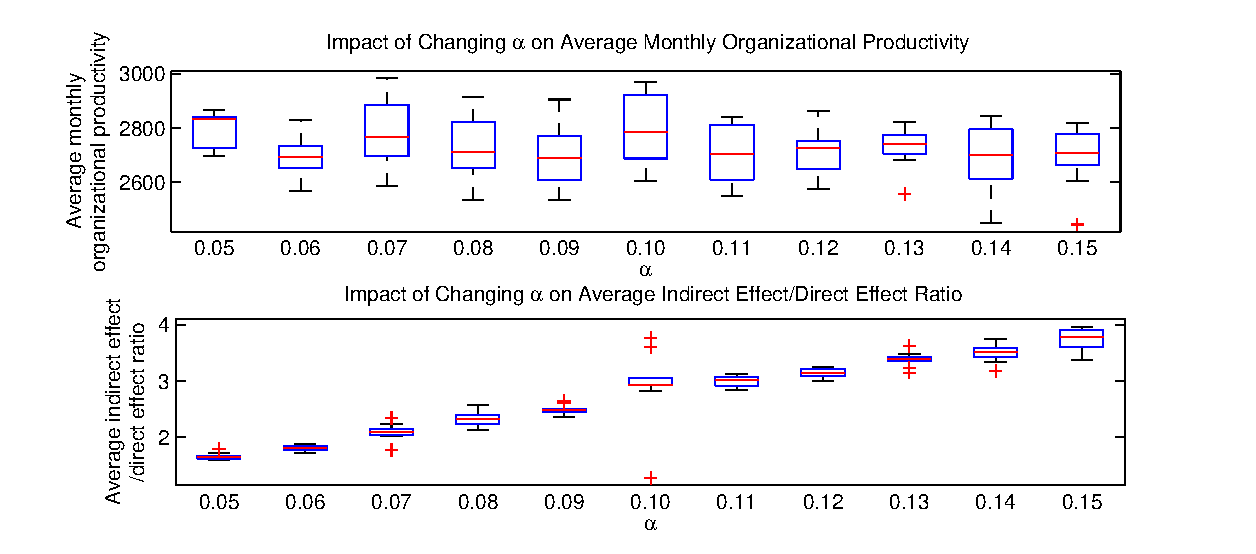
\includegraphics[width=16cm]{Sensitivity.eps}
\caption{Sensitivity Analysis on Parameter $\alpha$} 
\label{fig:2}
\end{figure}

As we can see, the productivity is insensitive to our parameter $\alpha$. A 50\% change in $\alpha$ will bring no more than 5\% change in calculated productivity in most cases. 

It is quite different if we look into the ratio between indirect effect and direct effect. It is actually sensitive to the change of $\alpha$. When $\alpha$ changes from 0.05 to 0.25, the median value of the ratio changes from less than 2 to nearly 4. However, we have valid reasons for this. Consider how this parameter acts in our model. It is actually a reflection of the psychological impact intensity for how the dissatisfaction in job affects a person's productivity. This impact, in reality, can come from shared cognition, the closeness between staff members, company morale and other subtle influence. Quite an amount of research has been done for tracking these influences.\cite{seligman2000positive}. So some empirical research may help when we want to determine the actual level of this parameter.

\section{Strengths and Weaknesses}

\subsection{Strengths}
\begin{itemize}
\item \textbf{Simplicity}: Our measures are based on easily understood principles and there are simple ways to compute them. In addition, we make minimum assumptions on individual characteristics: only $\alpha$ and $\beta$ are required for inference. 
\item \textbf{Parameters}: Most of our strategies are non-parametric, and the parameters of the churn model have nice properties, allowing for simple but effective parameter estimation, reducing the need of tuning to a minimum.
\item \textbf{Coverage}: Our model and measures are capable of simulating a large number of scenarios associated with different churn rates, various recruiting and/or promoting strategies.
\item \textbf{Flexibility}: Our model can be easily incorporated with other assumptions. For example, if we assume that an individual accumulates dissatisfaction even without external influence, our model can be modified to cover this assumption simply by increasing the $\beta$-to-$\alpha$ ratio every time period.
\item \textbf{Appealing simulation results}: The simulation results of our model are very appealing. Not only does it effectively reflect the current situation, but it presents insightful predictions for the effect of changes on company situation. In the case of Task 4, we discovered that higher churn rates leads to lower productivity-cost ratio. 
\item \textbf{Heuristics for HR}: HR can gain considerable heuristics from our paper, e.g. how to change recruiting strategies to sustain a required number of positions, and how to reduce churn rates by providing incentives for those who are likely to churn.

\end{itemize}

\subsection{Weaknesses}
\begin{itemize}
\item \textbf{Simulation volatility}: Although our model has nice statistical properties, results generated by different simulations suffer high volatility. One possible remedy is to increase the sampling time, which reduces outcome variance at the cost of computational resources.

\item \textbf{Unrealistic assumptions}: Some of our measures are based on unrealistic foundations, e.g. productivity increases linearly with training costs, employees have no inclination towards different positions, etc., which results in imperfect characterization for the corresponding problem.

\item \textbf{Incomplete assumptions}: There are also some other perspectives where we fail to consider, such as the positive effects of team cognition on productivity. 
\end{itemize}


\section{Conclusion}

We constrcted a Human Capital networkWe analyze the churn problem in ICM company 

we construct a Human Capital network according to the hierarchical organization structure of ICM and create a simple yet effective model to capture the dynamic processes, which includes organizational churn, promotion, and recruitment. For organizational churn, we propose and implement our *** model based on Bayesian learning principles, which estimates and updates the likelihood of individual churn using the Beta-Bernoulli distribution. Then we develop three promotion measures based on the priorities of experience, dissatisfaction, and centrality. Furthermore, we propose several methods to control the recruitment 

\bibliographystyle{plain}
\bibliography{reference.bib}

\end{document}
